\subsection{Factorisation et résolution triangulaire}
La factorisation ainsi que la résolution triangulaire utilisent le même graphe de tâches.
%
Les pages mémoires utilisées composants la matrice sont distribuée en respectant l'affinité mémoire des tâches associées.
%
Cette affinité est fournit par Taggre et correspond à une distribution à peu près équitable des pages mémoires au fil du déroulement du graphe.
%
Malheureusement, nous ne pouvons pas distribuer toutes les pages de manière optimale car il arrive que certaines pages soient utilisées par plusieurs tâches ayant des affinités mémoires différentes.
%
Dans un tel cas, nous choisissons de placer la page mémoire sur le banc NUMA ayant le plus de tâches.


% -------------------------------
%\subsubsection{Mémoire distribuée}
En mémoire distribuée, nous n'effectuons pas les mêmes calculs qu'en mémoire partagée, mais les accélérations obtenues nous donnerons une approximation des performances que nous pourrons obtenir.
%
Sur la machine Rostand, la factorisation atteint une accélération de 11,8 et la résolution triangulaire une accélération de 3,5.
%
Sur la machine Manumanu, cette accélération monte à 93 pour la factorisation (Fig.~\ref{fig:res_facto_mpi_manu}) et à 73 pour la résolution triangulaire (Fig.~\ref{fig:res_trsv_mpi_manu}).


%   (-_-)   %
\begin{figure}[!ht]
     \begin{center}
        \subfigure[Factorisation ILU(0).]{%
          \label{fig:res_facto_mpi_manumanu}
          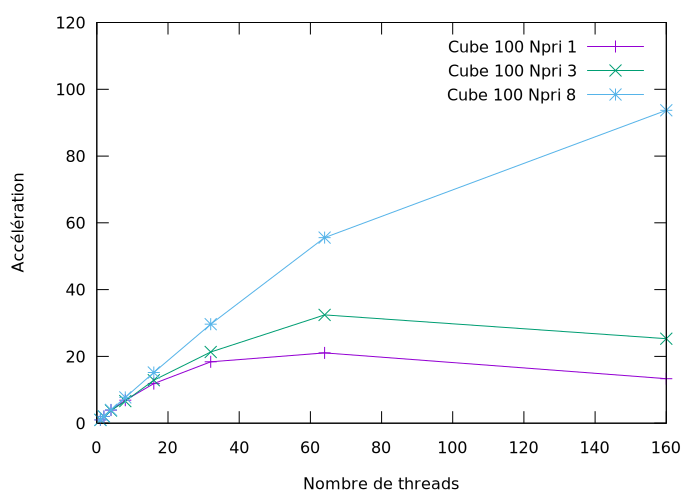
\includegraphics[width=0.49\textwidth]{res_facto_mpi_manu}
        }%
        \subfigure[Résolution triangulaire]{%
          \label{fig:res_trsv_mpi_manumanu}
          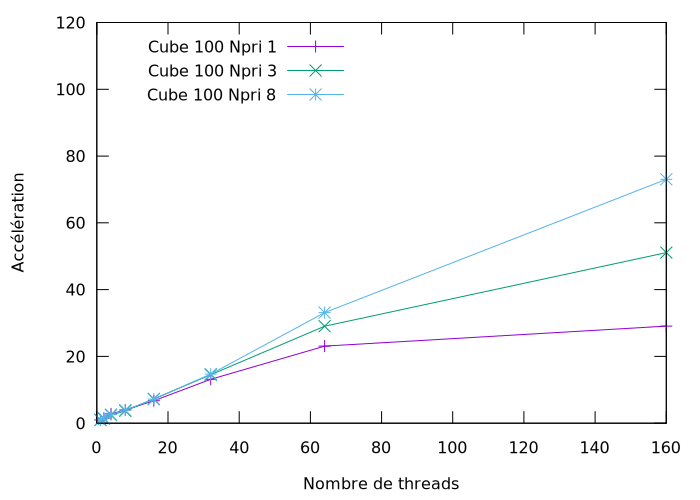
\includegraphics[width=0.49\textwidth]{res_trsv_mpi_manu}
        }%
    \end{center}
    \caption{Performances sur Manumanu en mémoire distribuée.}
\end{figure}

% -------------------------------
\subsubsection{First touch}
Les résultats de la factorisation et de la résolution triangulaire avec une allocation first touch sur la machine  sont exposés dans le chapitre précèdent.
%
Les résultats ne sont pas aussi bons que ceux que nous pourrions obtenir avec une meilleure gestion de la mémoire.
%
Pour rappel, nous obtenions au mieux une accélération de 8,7 sur coeurs pour la factorisation et une accélération de 2,8 pour la résolution triangulaire.


Sur la machine Manumanu, nous obtenons le même type d'accélération que pour le SpMV.
%
Tant que nous utilisons moins de 2 bancs NUMA, nous obtenons une accélération de 10 pour la factorisation (Fig.~\ref{fig:res_facto_ft_manumanu}) et une accélération de 6,2 pour la résolution triangulaire (Fig.~\ref{fig:res_trsv_ft_manumanu}).


%   (-_-)   %
\begin{figure}[!ht]
     \begin{center}
        \subfigure[Factorisation ILU(0).]{%
          \label{fig:res_facto_ft_manumanu}
          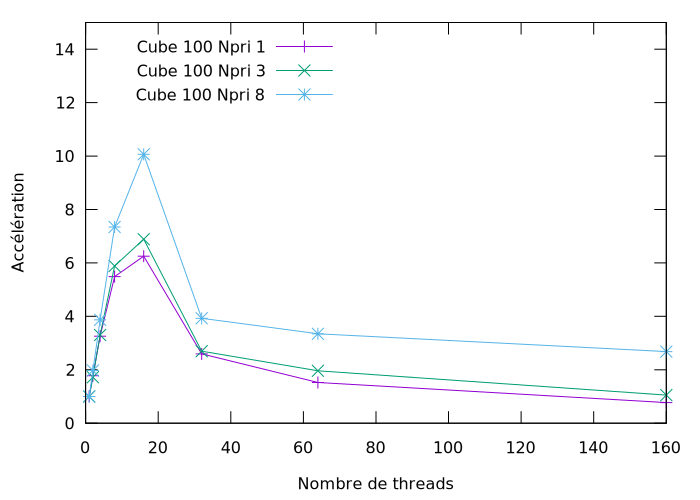
\includegraphics[width=0.49\textwidth]{res_facto_ft_manu}
        }%
        \subfigure[Résolution triangulaire]{%
          \label{fig:res_trsv_ft_manumanu}
          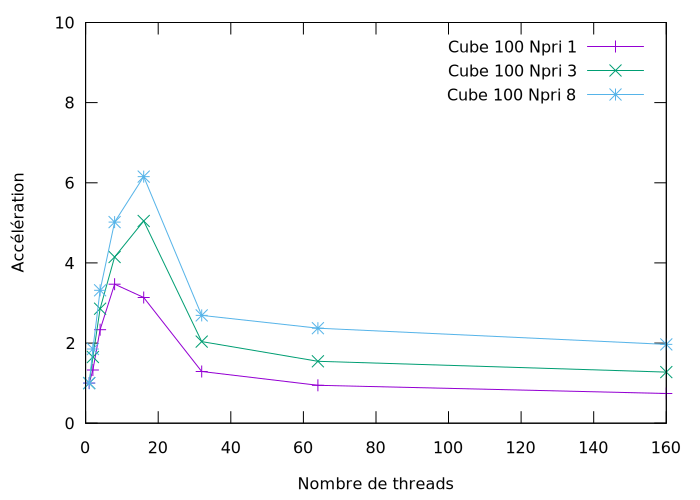
\includegraphics[width=0.49\textwidth]{res_trsv_ft_manu}
        }%
    \end{center}
    \caption{Performances sur Manumanu en utilisant une politique d'allocation first touch.}
\end{figure}

% -------------------------------
%\subsubsection{Interleave}
Pour essayer de diminuer les effets NUMA, nous activons la politique d'allocation mémoire interleave.
%
Les pages mémoires sont donc distribuées uniformément entre chaque banc NUMA.
%
Sur Rostand, la factorisation donne des résultats légèrement moins bons qu'avec une politique d'allocation first touch (Fig.~\ref{fig:res_facto_inter_rostand})
%
Par contre, nous obtenons une amélioration entre 3~\% et 30~\% de la résolution triangulaire pour un nombre faible de variables primaires (Fig.~\ref{fig:res_trsv_inter_rostand}).



%   (-_-)   %
\begin{figure}[!h]
     \begin{center}
        \subfigure[Factorisation ILU(0).]{%
          \label{fig:res_facto_inter_rostand}
          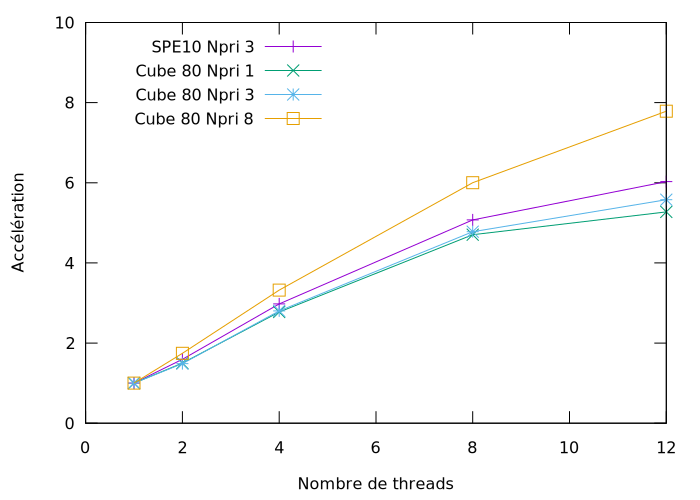
\includegraphics[width=0.49\textwidth]{res_facto_interleave}
        }%
        \subfigure[Résolution triangulaire]{%
          \label{fig:res_trsv_inter_rostand}
          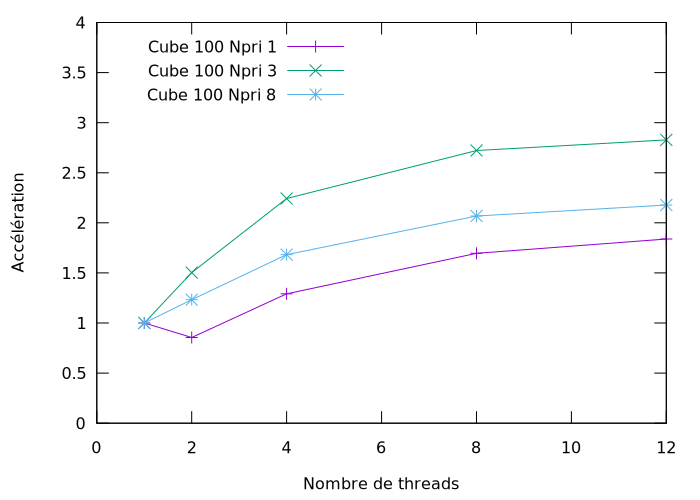
\includegraphics[width=0.49\textwidth]{res_trsv_interleave}
        }%
    \end{center}
    \caption{Performances sur Rostand en utilisant une politique d'allocation interleave.}
\end{figure}



Sur Manumanu, la factorisation se comporte de la même façon que sur Rostand (Fig.~\ref{fig:res_facto_inter_manumanu}).
%
De même, l'accélération maximale de la résolution triangulaire est meilleure avec une politique d'allocation interleave (Fig.~\ref{fig:res_trsv_inter_manumanu}).





%   (-_-)   %
\begin{figure}[!h]
     \begin{center}
        \subfigure[Factorisation ILU(0).]{%
          \label{fig:res_facto_inter_manumanu}
          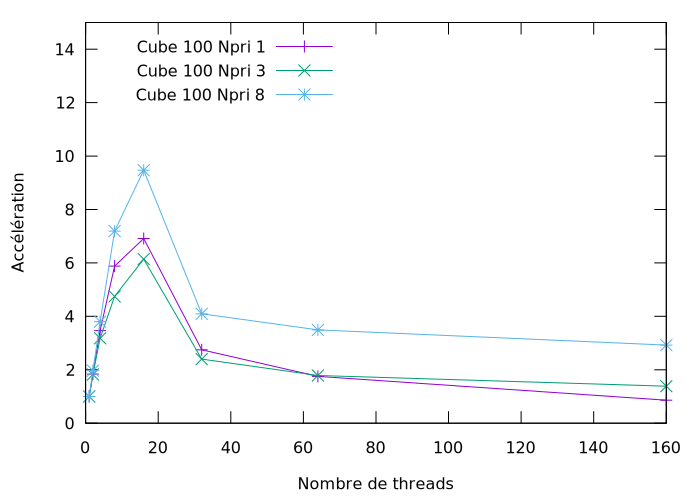
\includegraphics[width=0.49\textwidth]{res_facto_inter_manu}
        }%
        \subfigure[Résolution triangulaire]{%
          \label{fig:res_trsv_inter_manumanu}
          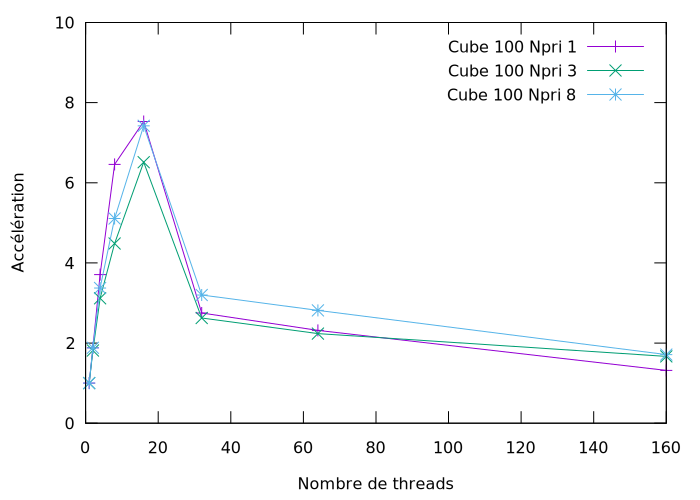
\includegraphics[width=0.49\textwidth]{res_trsv_inter_manu}
        }%
    \end{center}
    \caption{Performances sur Manumanu en utilisant une politique d'allocation interleave.}
\end{figure}

%-------------------------------
%\subsubsection{NATaS}
\`A la différence des autres ordonnanceurs, NATaS va tenir compte de l'affinité NUMA des tâches.
%
Cette affinité a été définit par Taggre de tel sorte à équilibrer la charge sur les différents bancs NUMA.
%
NATaS offre de meilleurs performances sur Rostand par rapport à la politique d'allocation interleave.
%
La factorisation est 40\% plus rapide avec 8 variables primaires et la résolution triangulaire est 23\% plus rapide.
%
Avec 1 variable primaire nous n'obtenons pas de gain sur la résolution triangulaire.


%   (-_-)   %
\begin{figure}[!ht]
     \begin{center}
        \subfigure[Factorisation ILU(0).]{%
          \label{fig:res_facto_nas_rostand}
          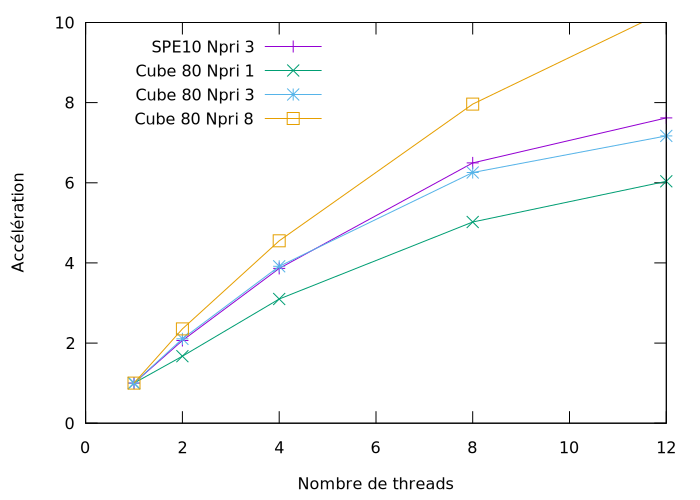
\includegraphics[width=0.49\textwidth]{res_facto_nas}
        }%
        \subfigure[Résolution triangulaire]{%
          \label{fig:res_trsv_nas_rostand}
          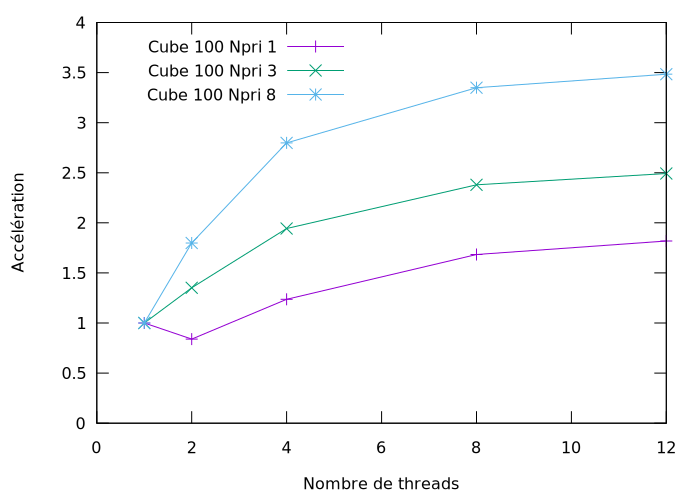
\includegraphics[width=0.49\textwidth]{res_trsv_nas}
        }%
    \end{center}
    \caption{Performances sur Rostand avec NATaS.}
\end{figure}



%   (-_-)   %
\begin{figure}[!ht]
     \begin{center}
        \subfigure[Factorisation ILU(0).]{%
          \label{fig:res_facto_nas_manu}
          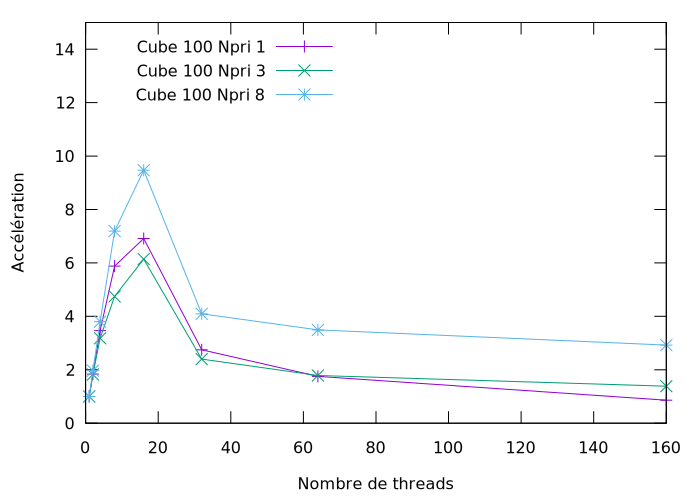
\includegraphics[width=0.49\textwidth]{res_facto_nas_manu}
        }%
        \subfigure[Résolution triangulaire]{%
          \label{fig:res_trsv_nas_manu}
          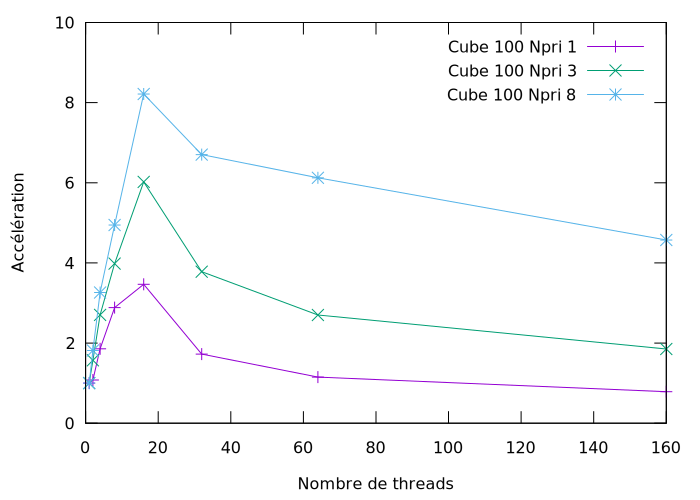
\includegraphics[width=0.49\textwidth]{res_trsv_nas_manu}
        }%
    \end{center}
    \caption{Performances sur Manu avec NATaS.}
\end{figure}

%-------------------------------
%\subsubsection{\'Equilibrage automatique NUMA}
L'équilibrage automatique des pages mémoires ne donne pas de bonnes performances sur la factorisation (Fig.~\ref{fig:res_facto_frep}).
%
Cette méthode d'allocation est la moins efficace de toutes.
%
Avec un nombre suffisant d'itérations, l'allocation interleave donne les mêmes performances que l'allocation first touch.
%
L'utilisation de NATaS reste la solution qui donne les meilleures performances.

%   (-_-)   %
\begin{figure}
  \centering
  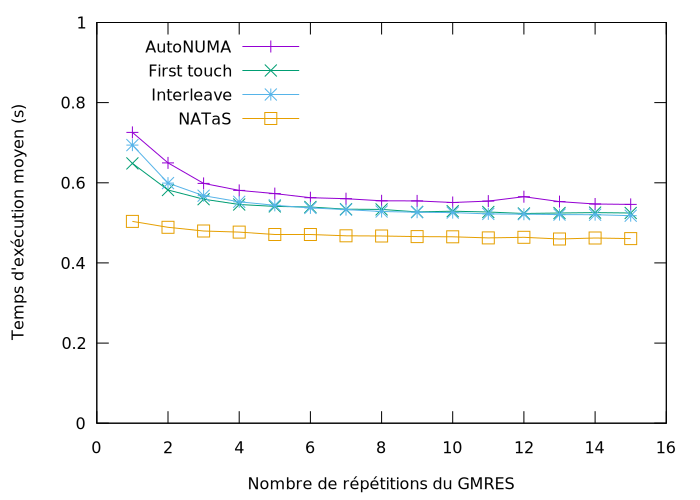
\includegraphics[width=0.7\textwidth]{res_facto_frep}
  \caption{Temps moyen d'une factorisation sur Linux 3.18 en mémoire partagée avec 12 coeurs. Nous utilisons une matrice représentant un cube 100 avec 8 variables primaires.}
  \label{fig:res_facto_frep}
\end{figure}
Par contre, la résolution triangulaire se comporte comme le SpMV (Fig.~\ref{fig:res_trsv_frep}).
%
La politique d'allocation autoNUMA offre des performances intermédiaires aux politiques d'allocations first touch et interleave.
%
Encore une fois, l'utilisation de NATaS est la plus efficace.

%   (-_-)   %
\begin{figure}
  \centering
  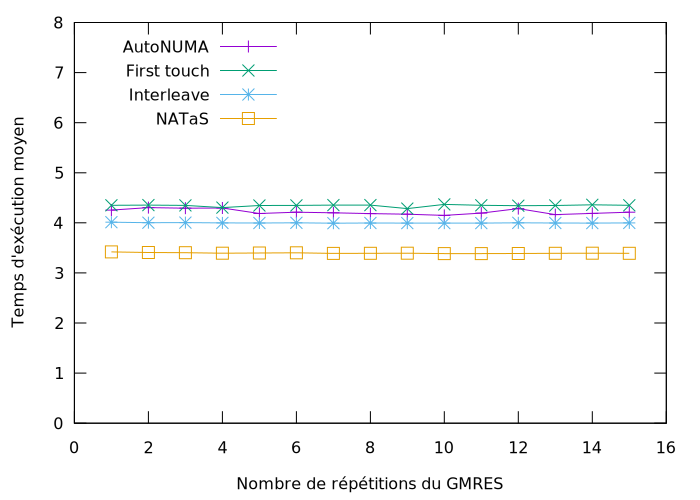
\includegraphics[width=0.7\textwidth]{res_trsv_frep}
  \caption{Temps moyen d'une résolution triangulaire sur Linux 3.18 en mémoire partagée avec 12 coeurs. Nous utilisons une matrice représentant un cube 100 avec 8 variables primaires.}
  \label{fig:res_trsv_frep}
\end{figure}

% -------------------------------
